% *********************************************************************
% © 2010–2026 Jeremy Sylvestre
%
% Permission is granted to copy, distribute and/or modify this document
% under the terms of the GNU Free Documentation License, Version 1.3 or
% any later version published by the Free Software Foundation; with no
% Invariant Sections, no Front-Cover Texts, and no Back-Cover Texts. A
% copy of the license is included in the appendix entitled “GNU Free
% Documentation License” that appears in the output document of this
% PreTeXt source code. All trademarks™ are the registered® marks of
% their respective owners.
%
% *********************************************************************

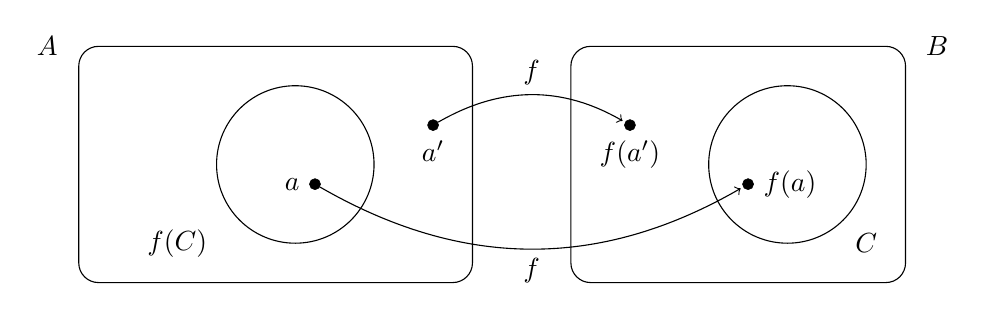
\begin{tikzpicture}[
	vertex/.style={ circle, draw, very thin, fill, inner sep=0pt, minimum size=4pt },
	vertexg/.style={ black!40!white, circle, draw, very thin, fill, inner sep=0pt, minimum size=4pt },
	vertexo/.style={ circle, draw, very thin, inner sep=0pt, minimum size=4pt }
]

\draw (-4.5,1.5) -- (-6.25,1.5)
	arc (90:180:0.25cm) -- (-6.5,-1.25)
	arc (180:270:0.25cm) -- (-1.75,-1.5)
	arc (270:360:0.25cm) -- (-1.5,1.25)
	arc (0:90:0.25cm) -- (-4.5,1.5);
\node at (-6.9,1.5) {$A$};
\draw (2.5,1.5) -- (3.75,1.5)
	arc (90:0:0.25cm) -- (4,-1.25)
	arc (360:270:0.25cm) -- (0,-1.5)
	arc (270:180:0.25cm) -- (-0.25,1.25)
	arc (180:90:0.25cm) -- (2.5,1.5);
\node at (4.4,1.5) {$B$};
\draw (-3.75,0) circle (1cm);
\node at (-5.25,-1) {$\inv{f}(C)$};
\draw (2.5,0) circle (1cm);
\node at (3.5,-1) {$C$};
\node at (-3.5,-0.25) (a) [vertex,label=left:{$a$}] {};
\node at (2,-0.25) (b) [vertex,label=right:{$f(a)$}] {};
\draw[->,shorten >=1pt] (a) to [out=-30,in=-150] node[below] {$f$} (b);
\node at (-2,0.5) (x) [vertex,label=below:{$a'$}] {};
\node at (0.5,0.5) (y) [vertex,label=below:{$f(a')$}] {};
\draw[->,shorten >=1pt] (x) to [out=30,in=150] node[above] {$f$} (y);

\end{tikzpicture}
